 \documentclass[a4paper,10pt]{article}
\input{/Users/WannaGetHigh/workspace/latex/macros.tex}

\title{TP - TI : images discr�tes}
\author{Fran�ois \bsc{Lepan}}

\begin{document}
\maketitle

\section{Composantes d'une image couleur}

\subsection{Quelle sont les dimensions de la variable utilis�e pour stocker l'image et que repr�sentent-t-elles?}

Les dimensions de l'image sont �gales a sa taille en pixels x le nombre de couleur (ici 800x600x3). \\ 

Pour un �l�ment se situant a (23,23,z) de la matrice:\\
	la valeur z = 1 correspond a la quantit� de rouge du pixel (23, 23) \\
	la valeur z = 2 correspond a la quantit� de vert du pixel (23, 23) \\
	la valeur z = 3 correspond a la quantit� de bleu du pixel (23, 23) \\

\subsection{S�parer les composantes rouge, verte et bleue}

\begin{paragraph}{En niveau de gris}
\begin{verbatimtab}
img = imread("ti-semaine-3-mire.png");

// recupere les niveaux de gris pour la couleur rouge 
imgRG = img(:,:,1);
// recupere les niveaux de gris pour la couleur bleu 
imgGG = img(:,:,2);
// recupere les niveaux de gris pour la couleur vert 
imgBG = img(:,:,3);
// affichage
imshow([imgRG, imgGG, imgBG]);
\end{verbatimtab}
\end{paragraph}

L'ex�cution du code pr�c�dent fournit la Fig.~\ref{fig:niveau_de_gris_composante_RGB} sur laquelle on peut observer de gauche � droite les niveaux de gris pour la couleur rouge puis vert puis bleu.

\begin{figure}[ht]
	\begin{center}
		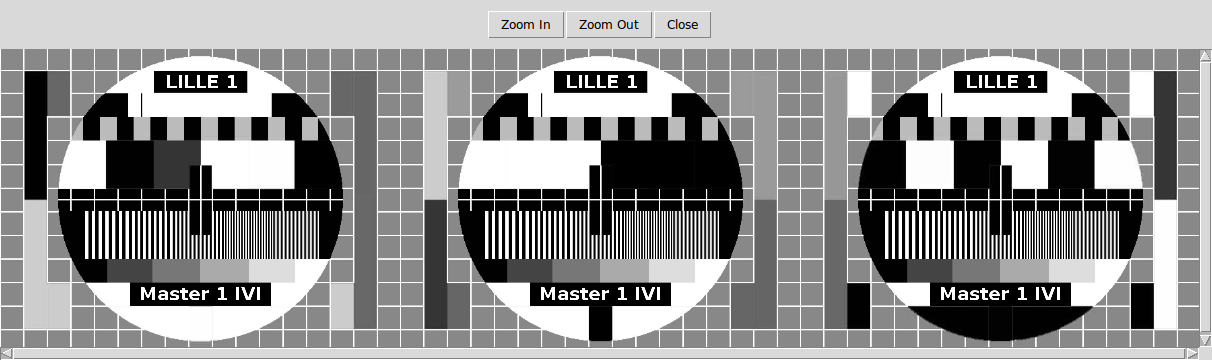
\includegraphics[width=15cm]{niveau_de_gris_composante_RGB.png}
	\end{center}
	\caption{Niveau de gris de gauche � droite des couleurs rouge, vert et bleu}
	\label{fig:niveau_de_gris_composante_RGB}
\end{figure}

\newpage

\begin{paragraph}{En couleur}
Voici le code correspondant a la s�paration des trois composantes:
\begin{verbatim}
function imgR = redColorsOf(img)
    imgR = img;
    imgR(:,:,2) = img(:,:,1)*0;
    imgR(:,:,3) = img(:,:,1)*0;
endfunction

function imgG = greenColorsOf(img)
    imgG = img;
    imgG(:,:,1) = img(:,:,1)*0;
    imgG(:,:,3) = img(:,:,1)*0;
endfunction

function imgB = blueColorsOf(img)
    imgB = img;
    imgB(:,:,1) = img(:,:,1)*0;
    imgB(:,:,2) = img(:,:,1)*0;
endfunction

img = imread("ti-semaine-3-mire.png");

// met les valeur pour le vert et le bleu a 0
imgR = redColorsOf(img);
// met les valeur pour le rouge et le bleu a 0
imgG = greenColorsOf(img);
// met les valeur pour le vert et le rouge a 0
imgB = blueColorsOf(img);
// affichage
imshow([imgR, imgG, imgB]);
\end{verbatim}

L'ex�cution du code pr�c�dent fournit la Fig.~\ref{fig:couleur_composante_RGB} sur laquelle on peut observer de gauche � droite les composantes couleur rouge puis vert puis bleu.

\begin{figure}[ht]
	\begin{center}
		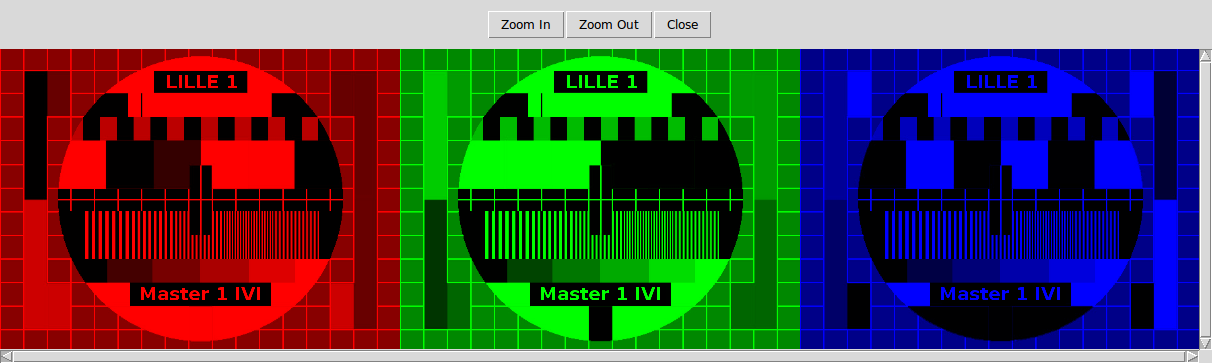
\includegraphics[width=15cm]{couleur_composante_RGB.png}
	\end{center}
	\caption{Les composantes couleur rouge puis vert puis bleu.}
	\label{fig:couleur_composante_RGB}
\end{figure}

\end{paragraph}


\begin{paragraph}{V�rification de la r�cup�ration de l'image pour les trois composante}
\begin{verbatim}
imgRes = img;
imgRes = img(:,:,1)*0;
imgRes = img(:,:,2)*0;
imgRes = img(:,:,3)*0;
imgRes(:,:,1) = imgR(:,:,1);
imgRes(:,:,2) = imgG(:,:,2);
imgRes(:,:,3) = imgB(:,:,3);
imshow(imgRes);
\end{verbatim}

L'ex�cution du code pr�c�dent fournit la Fig.~\ref{fig:ti-semaine-3-mire}  qui est l'addition des trois composantes couleur rouge puis vert puis bleu de la Fig.~\ref{fig:couleur_composante_RGB}.

\begin{figure}[ht]
	\begin{center}
		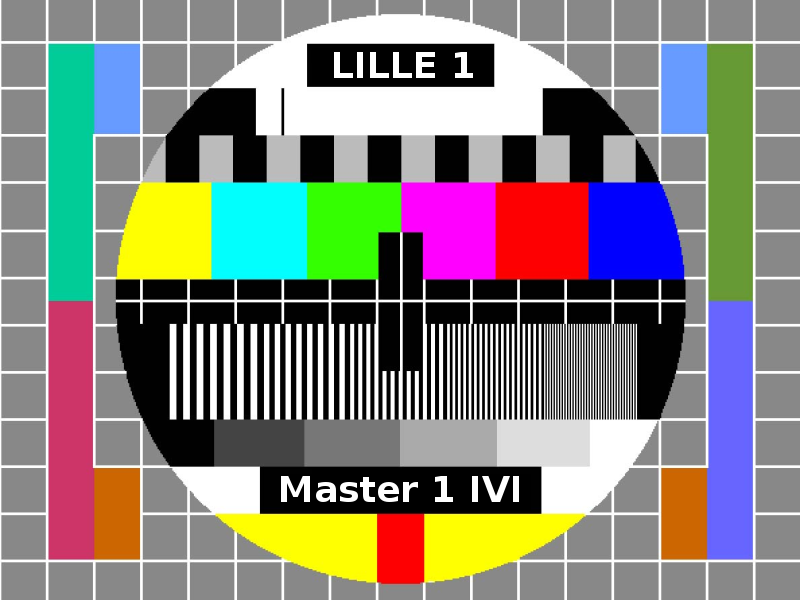
\includegraphics[width=8cm]{ti-semaine-3-mire.png}
	\end{center}
	\caption{Image de base}
	\label{fig:ti-semaine-3-mire}
\end{figure}


\end{paragraph}

\section{Sur et sous-�chantillonnage}

\section {Quantification}

\section {Repliement de spectre}



\end{document}